\documentclass[../xlapes02]{subfiles}
\begin{document}
    \chapter{Implementation}\label{ch:implementation}


    \section{Data Engineering}\label{sec:data-engineering}
    Data engineering is critical in AI to ensure data quality, preparation, integration, scalability, governance, and performance optimization. It involves cleaning, organizing, and transforming data for accurate model training, handling large volumes of data, and adhering to regulations. High-quality data and effective data engineering processes are crucial for developing reliable and scalable AI models. In this section, we describe our approach to data engineering used for Portfolio Management by first defining the data collection~\cref{subsec:data-collection}, dataset preprocessing~\cref{subsec:dataset-preprocessing}, and dataset splitting~\cref{subsec:dataset-splitting}.

    \subsection{Data Collection}\label{subsec:data-collection}
    Raw data was gathered from these sources:
    \begin{itemize}
        \item Yahoo Finance: \url{https://finance.yahoo.com/}
        \item Financial Modeling Prep: \url{https://financialmodelingprep.com/}
    \end{itemize}
    these sources provide financial data for 60000+ tickers, with a history of over 30 years.

    We focus on tickers (companies) from Dow Jones Industrial Average (DJIA), which includes 30 companies. More about which companies are included in DJIA, you can see~\cite{enwiki:1141766585}.

    \subsection{Data Preprocessing}\label{subsec:dataset-preprocessing}
    In this section, we describe our approach to dataset preprocessing by first defining the data cleaning~\cref{subsubsec:data-cleaning}, feature engineering~\cref{subsubsec:feature-engineering}.

    \subsubsection{Data Cleaning}\label{subsubsec:data-cleaning}
    In our datasets, we use the following companies' data: prices, financial statements, and technical indicators. The prices are used for calculating the returns, the financial statements are used for calculating the financial ratios, and the technical indicators are used for calculating the technical ratios. The financial and technical ratios are used for feature engineering. The data cleaning is done by removing the rows with missing values. The missing values are replaced with the mean of the column. If on any date the data is missing completely, then all rows until that next date are removed for other companies as well. This can mostly happen for companies that are not listed on the stock exchange for any time period. The data cleaning is done for all the datasets.

    \subsection{Feature Engineering}\label{subsubsec:feature-engineering}
    In this subsection, we describe our approach to feature engineering which we divide into three parts: fundamental analysis, described in~\cref{subsubsec:fundamental-analysis}, technical analysis, described in~\cref{subsubsec:technical-analysis}, and combined fundamental and technical analysis is described in~\cref{subsubsec:combined-fundamental-and-technical-analysis}.

    \subsubsection{Fundamental Analysis}\label{subsubsec:fundamental-analysis}
    Fundamental data refers to the basic and essential information about a company or an asset that is used to analyze its financial health, performance, and valuation. It includes data related to a company's financial statements, business operations, management team, industry, and economic environment. Fundamental data is commonly used by investors, analysts, and financial professionals to make investment decisions and assess the intrinsic value of an asset. For fundamental analysis, we use the following Income Statement, Balance Sheet, and Cash Flow of each company. For our first dataset, we use the following financial ratios: Net Profit Margin. Return on Assets (ROA), Return on Equity (ROE), Current Ratio, Cash Ratio, Inventory Turnover, Receivables Turnover, Payables Turnover, Debt Ratio, Debt to Equity Ratio, A Price to Earnings Ratio (PE Ratio), Price to Book Ratio (PB Ratio), and Dividend Yield. Now we describe each of these ratios.

    \paragraph{Net Income}\label{par:net-income}
    Net income is the amount of money a company makes after subtracting all expenses and taxes. It is also known as the bottom line because it is found on the last line of a company's income statement. The Net Income is calculated as:
    \begin{equation}
        \begin{split}
            Net\ Income&=R-COGS-E-I-T\\
        \end{split}
    \end{equation}
    where $R$ is the revenue, $COGS$ is the cost of goods sold, $E$ is the expenses, $I$ is the interest, and $T$ is the taxes.

    \paragraph{Operating Profit Margin}\label{par:operating-profit-margin}
    The Operating Margin represents how efficiently a company is able to generate profit through its core operations. It is expressed on a per-sale basis after accounting for variable costs but before paying any interest or taxes (EBIT). Higher margins are considered better than lower margins and can be compared between similar competitors but not across different industries. To calculate the operating margin, divide operating income (earnings) by sales (revenues)~\cite{investopedia-operating-margin}:
    \begin{equation}
        Operating\ Margin=\frac{Operating\ Income}{Sales}
    \end{equation}
    where $Operating\ Income$ refers to the adjusted revenue of a company after all expenses of operation and depreciation are subtracted. Expenses of operation or operating expenses are simply the costs incurred in order to keep the business running~\cite{investopedia-operating-income}. $Sales$ may be defined as money paid by customers. Sales are a company's core revenue for a given period~\cite{investopedia-operating-margin}.

    \paragraph{Net Profit Margin}\label{par:net-profit-margin}
    The Net Profit Margin is a profitability ratio that measures a company's ability to generate income after all expenses and taxes have been paid. It is calculated by dividing a company's net income by its total revenue. The net profit margin is a measure of how much of each dollar of revenue is left over after all expenses and taxes have been paid. It is a useful metric for comparing the profitability of different companies in the same industry. The higher the net profit margin, the more profitable a company is. The net profit margin is calculated as follows~\cite{investopedia-net-profit-margin}.:
    \begin{equation}
        \begin{split}
            Net\ Profit\ Margin&=\frac{Net\ Income}{Revenue}\\
        \end{split}
    \end{equation}

    \paragraph{Return On Assets}\label{par:return-on-assets}
    Return on assets (ROA) is a measure of profitability that calculates how much profit a company makes with the money it has invested. It is calculated by dividing a company's net income by its total assets. The higher the ROA, the more profitable a company is. The ROA is calculated as follows~\cite{investopedia-return-on-assets}:
    \begin{equation}
        \begin{split}
            Return\ On\ Assets&=\frac{Net\ Income}{Total\ Assets}\\
        \end{split}
    \end{equation}

    \paragraph{Return On Equity}\label{par:return-on-equity}
    Return on equity (ROE) is a measure of profitability that calculates how much profit a company makes with the money shareholders have invested. It is calculated by dividing a company's net income by its shareholders' equity. The higher the ROE, the more profitable a company is. The ROE is calculated as follows~\cite{investopedia-return-on-equity}:
    \begin{equation}
        \begin{split}
            Return\ On\ Equity&=\frac{Net\ Income}{Average Shareholders'\ Equity}\\
        \end{split}
    \end{equation}

    \paragraph{Current Ratio}\label{par:current-ratio}
    The current ratio is a liquidity ratio that measures a company's ability to pay short-term and long-term obligations. It is calculated by dividing a company's current assets by its current liabilities. The higher the current ratio, the more capable a company is of paying its short-term and long-term obligations. The current ratio is calculated as follows~\cite{investopedia-current-ratio}:
    \begin{equation}
        \begin{split}
            Current\ Ratio&=\frac{Current\ Ratio}{Debt+Other\ Payables}\\
        \end{split}
    \end{equation}
    where $Current\ Ratio$ is $Cash\&Equivalent+Short\ Term\ Investments+Account\ Receivable+Inventory$. If the $Current Ratio < 1$ that is a sign of financial distress, and the company could be unable to pay its short-term and long-term obligations. On the other hand, if the $Current Ratio$ is too high, it could be a sign that the company is not using its assets efficiently.

    \paragraph{Quick Ratio}\label{par:quick-ratio}
    The quick ratio is a liquidity ratio that measures a company's ability to pay short-term obligations. It is calculated by dividing a company's quick assets by its current liabilities. The higher the quick ratio, the more capable a company is of paying its short-term obligations. The quick ratio is calculated as follows~\cite{investopedia-quick-ratio}:
    \begin{equation}
        \begin{split}
            Quick\ Ratio&=\frac{Cash\&Equivalent+Short\ Term\ Investments+Account\ Receivable}{Current\ Liabilities}\\
        \end{split}
    \end{equation}
    If the company would have a $Quick Ratio < 1$, it would be a sign of financial distress, and the company would be unable to pay its short-term obligations.

    \paragraph{Cash Ratio}\label{par:cash-ratio}
    The cash ratio is a liquidity ratio that measures a company's ability to pay short-term obligations. It is calculated by dividing a company's cash and cash equivalents by its current liabilities. The higher the cash ratio, the more capable a company is of paying its short-term obligations. The cash ratio is calculated as follows~\cite{investopedia-cash-ratio}:
    \begin{equation}
        \begin{split}
            Cash\ Ratio&=\frac{Cash\&Equivalent}{Current\ Liabilities}\\
        \end{split}
    \end{equation}

    \paragraph{Inventory Turnover}\label{par:inventory-turnover}
    The inventory turnover ratio is a measure of how efficiently a company is managing its inventory. It is calculated by dividing a company's cost of goods sold by its average inventory. The higher the inventory turnover ratio, the more efficiently a company is managing its inventory. The inventory turnover ratio is calculated as follows~\cite{investopedia-inventory-turnover}:
    \begin{equation}
        \begin{split}
            Inventory\ Turnover&=\frac{Cost\ of\ Goods\ Sold}{Average\ Inventory}\\
        \end{split}
    \end{equation}

    \paragraph{Receivables Turnover}\label{par:receivables-turnover}
    The receivables turnover ratio is a measure of how efficiently a company is managing its accounts receivable. It is calculated by dividing a company's net credit sales by its average accounts receivable. The higher the receivables turnover ratio, the more efficiently a company is managing its accounts receivable. The receivables turnover ratio is calculated as follows~\cite{investopedia-recievables-turnover}:
    \begin{equation}
        \begin{split}
            Receivables\ Turnover&=\frac{Net\ Credit\ Sales}{Average\ Accounts\ Receivable}\\
        \end{split}
    \end{equation}

    \paragraph{Payables Turnover}\label{par:payables-turnover}
    The payables turnover ratio is a measure of how efficiently a company is managing its accounts payable. It is calculated by dividing a company's cost of goods sold by its average accounts payable. The higher the payables turnover ratio, the more efficiently a company is managing its accounts payable. The payables turnover ratio is calculated as follows~\cite{investopedia-payables-turnover}:
    \begin{equation}
        \begin{split}
            Payables\ Turnover&=\frac{TSP}{(BAP+EAP)/2}\\
        \end{split}
    \end{equation}
    where $TSP$ is the total supply purchase, $BAP$ is the beginning accounts payable, and $EAP$ is the ending accounts payable. If the payables turnover ratio is too low, it could be a sign that company has trouble paying its suppliers. If the payables turnover ratio is too high, it could be a sign that the company is not using its assets efficiently.

    \paragraph{Debt Ratio}\label{par:debt-ratio}
    The debt ratio is a measure of a company's financial leverage. It is calculated by dividing a company's total liabilities by its total assets. The higher the debt ratio, the more debt a company is using to finance its assets. The debt ratio is calculated as follows~\cite{investopedia-debt-ratio}:
    \begin{equation}
        \begin{split}
            Debt\ Ratio&=\frac{Traditional\ Debt+(Accounts\ Payable+Taxes\ Payable)}{Total Assets}\\
        \end{split}
    \end{equation}
    The lower the debt ratio, the better. A $Debt\ Ratio > 1.0$ means a company has more debt than assets while a $Debt\ Ratio < 1$ indicates that a company has more assets than debt.

    \paragraph{Debt Equity Ratio}\label{par:debt-equity-ratio}
    The debt equity ratio is a measure of a company's financial leverage. It is calculated by dividing a company's total liabilities by its total equity. The higher the debt equity ratio, the more debt a company is using to finance its assets. The debt equity ratio is calculated as follows~\cite{investopedia-debt-equity-ratio}:
    \begin{equation}
        \begin{split}
            Debt\ Equity\ Ratio&=\frac{Traditional\ Debt+(Accounts\ Payable+Taxes\ Payable)}{Total\ Equity}\\
        \end{split}
    \end{equation}

    \paragraph{Price Earnings Ratio}\label{par:price-earnings-ratio}
    The price earnings ratio is a measure of a company's value relative to its earnings. It is calculated by dividing a company's stock price by its earnings per share. The higher the price earnings ratio, the more expensive a company's stock is relative to its earnings. The price earnings ratio is calculated as follows~\cite{investopedia-price-earnings-ratio}:
    \begin{equation}
        \begin{split}
            Price\ Earnings\ Ratio&=\frac{Stock\ Price}{Earnings\ Per\ Share}\\
        \end{split}
    \end{equation}

    \paragraph{Price Book Value Ratio}\label{par:price-book-value-ratio}
    The price book value ratio is a measure of a company's value relative to its book value. It is calculated by dividing a company's stock price by its book value per share. The higher the price book value ratio, the more expensive a company's stock is relative to its book value. The price book value ratio is calculated as follows~\cite{investopedia-price-book-value-ratio}:
    \begin{equation}
        \begin{split}
            Price\ Book\ Value\ Ratio&=\frac{Stock\ Price}{Book\ Value\ Per\ Share}\\
        \end{split}
    \end{equation}

    \paragraph{Dividend Yield}\label{par:dividend-yield}
    The dividend yield is a measure of a company's profitability. It is calculated by dividing a company's annual dividend by its stock price. The higher the dividend yield, the more profitable a company is. The dividend yield is calculated as follows~\cite{investopedia-dividend-yield}:
    \begin{equation}
        \begin{split}
            Dividend\ Yield&=\frac{Annual\ Dividend}{Stock\ Price}\\
        \end{split}
    \end{equation}

    \subsubsection{Technical Analysis}\label{subsubsec:technical-analysis}
    Technical analysis is a method used in financial markets such as stocks, currencies and commodities to analyse historical price data and identify patterns, trends and signals that can be used to make trading decisions. Technical analysis is based on the belief that historical price and volume data can provide insight into future price movements and focuses primarily on the analysis of price charts and other technical indicators. In this section we present the technical indicators that we have selected based on the correlation matrix between all indicators.


    \section{Feature Selection}\label{sec:feature-selection}
    The technical indicators are calculated based on the historical data of the stock prices. For calculation of these indicator was used framework Finta, which provides over 80 different functions for calculation of technical indicators. The framework is written in Python and is available on GitHub~\cite{finta}.

    Firstly we compute all technical indicators for all stocks in the dataset. Then we compute the correlation matrix between all indicators. The correlation matrix is a square matrix that contains the correlation coefficient between all pairs of indicators. The correlation coefficient is a measure of the linear correlation between two variables. The corelation drop coefficient is $0.5$, when $|\rho| > 0.5$, then we drop the one indicator, where $\rho$ is the correlation between two indicators, defined in~\cref{eq:corr}. Because the figure for all indicators is too large, we only show the correlation matrix for uncorrelated indicators, which we used in dataset, see ~\cref{fig:ta_correlation_matrix_uncorrelated_indicators}.
    \begin{figure}[h]
        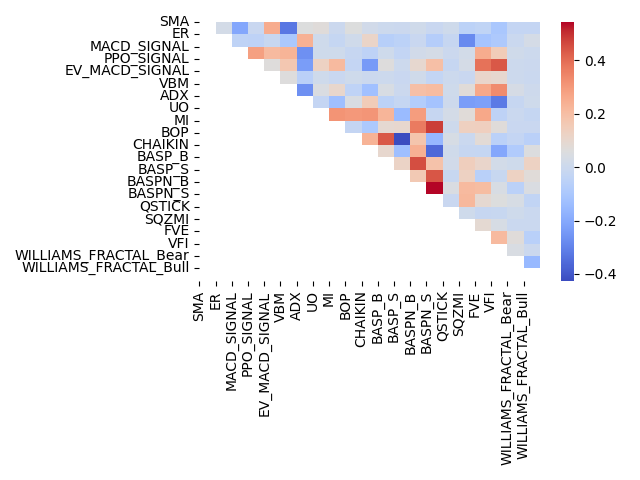
\includegraphics[width=0.95\linewidth]{image/ta_correlation_matrix_uncorrelated_indicators}
        \centering
        \caption{Correlation matrix of technical indicators after removing correlated indicators.}
        \label{fig:ta_correlation_matrix_uncorrelated_indicators}
    \end{figure}

    The correlation coefficient $\rho$ is calculated using \emph{Pearson Method} as follows~\cite{enwiki:1146097966}:
    \begin{equation}
        \label{eq:corr}
        \begin{split}
            \rho&=\frac{\sum_{i=1}^{n}(x_i-\bar{x})(y_i-\bar{y})}{\sqrt{\sum_{i=1}^{n}(x_i-\bar{x})^2}\sqrt{\sum_{i=1}^{n}(y_i-\bar{y})^2}}\\
        \end{split}
    \end{equation}

    \subsubsection{Combined Fundamental and Technical Analysis}\label{subsubsec:combined-fundamental-and-technical-analysis}
    The combined fundamental and technical analysis is a combination of fundamental and technical analysis features. The fundamental analysis is described in \cref{subsubsec:fundamental-analysis} and the technical analysis is described in \cref{subsubsec:technical-analysis}.

    \subsection{Dataset Splitting}\label{subsec:dataset-splitting}
    The dataset is split into two parts: training and testing. Since the dataset it timeseries data, we divide it based on that. The division coefficient is $0.6$.
    The $60\%$ of data is for training and the $40\%$ of data is for testing. The dataset starts at 2008-03-20 and ends at 2022-12-16.
    Dataset consists of daily data.


\end{document}
